\chapter{Semantic Triple Extraction Engine}

\vspace{-2ex}
This section focuses on the Semantic Triple Extraction Engine, focusing on triple representation and the different approaches of information extraction.

\section{Motivation}
The aim of this engine was to find a way to extract meaningful information from the article, in particular, information centred around key entities in the article corpus for a certain topic. One of the earlier approaches was to derive a co-occurrence graph of named entities of type 'GPE', 'PER', 'LOC', 'ORG' etc. (using Fine-Grained NER~\Cref{s:models}) for a topic. The limitation of this approach, was that while it was a good indicator of general entities in a topic, the amount of information extracted from the topic article corpus was not sufficient as no explicit information about \textit{`how'} the entities were related to one another was inferred. In an attempt to extract more 'relevant' information indicative to the content discussed in articles of a given topic, the decision was made to extract semantic triples of type \texttt{subject-predicate-object}. The triple serves as a minimal representation for information in an artcile without losing the context. The process of extracting these relations involved inferring both syntactic and semantic dependencies between tokens in a sentence, making use tokenisation, dependency parsing,  part-of-speech tagging and named entity recognition. These triples would then be displayed as a knowledge graph (Refer to \Cref{Knowledge_graph}) for each topic in a semantic cluster.

\section{Key decisions} \label{key_decisions_rel}

In an attempt to capture meaningful nodes (subjects and objects) and relations (predicate), the Semantic Triple Extraction Engine uses phrases instead of words. \Cref{fig:rel_key_decisions} shows the 3 main decisions made for the representation of the triples. 

\begin{figure}[H]
  \centering
  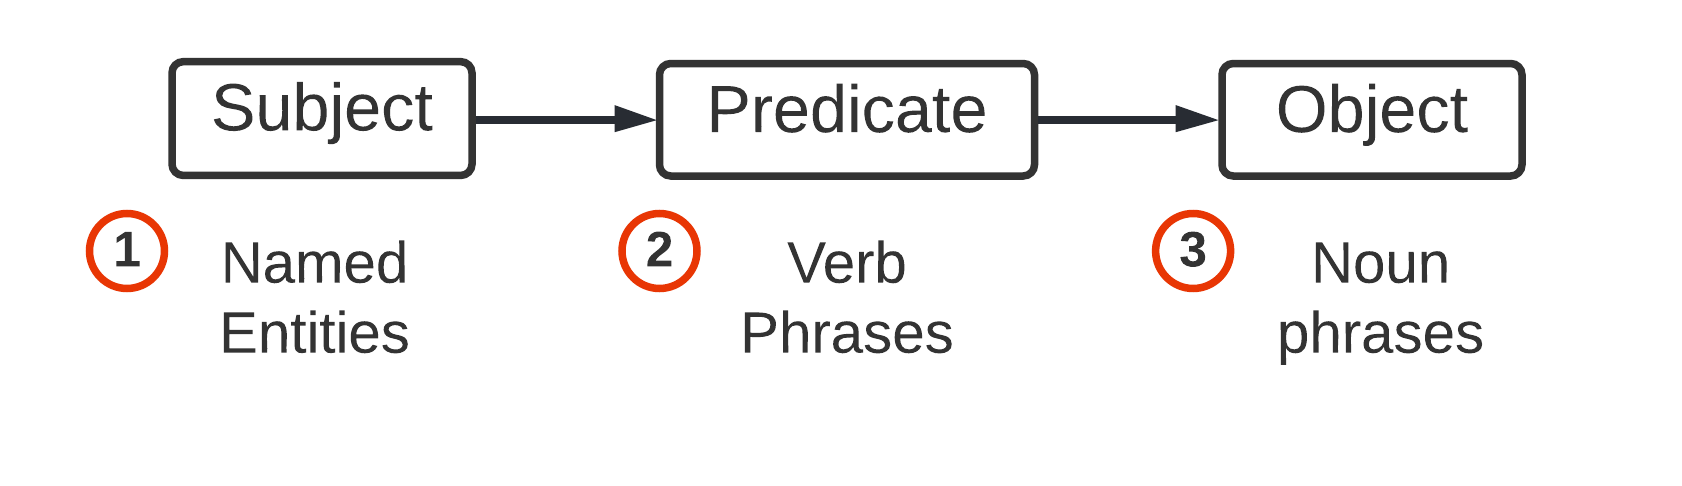
\includegraphics[scale=0.15]{images/relations_kd.png}
  \caption{Decisions for Extracting Semantic Triples}
  \vspace{-1ex}
  \label{fig:rel_key_decisions}
\end{figure}

\begin{enumerate}
  \item \textbf{Named Entities as Subjects:} Given that the end goal is to build a knowledge graph (KG) from these triples, there need to be common `subject' nodes in order to infer information about these entities from the articles, link them to other entities in the graph. For example, if the subject requirement is changed from named entities to simply noun phrases, the engine might extract two triples: one with subject `British Airways' and another with `British Airways spokesperson'. This is not ideal as, although both triples provide information about the named entity `British Airways', they will be displayed as discrete triples. Therefore, using `named entities' as subject grounds the KG to a set of named entities, for which information (semantic triples) can be extracted.
  
  \item \textbf{Verb Phrases as Predicate:} Based on the success of previous studies ~\cite{verb_relation_extraction}, the engine relies on the verb-based approach for predicate extraction. It aims to extract a single relation embedded in a sentence that consists of a verb phrase sandwiched between two entities of interest. The motivation for using verb phrases as predicate is that it exploits the structured grammar present in news articles where generally the subject is usually a person, organisation, place or thing (hence, the use of named entities) and the predicate indicates what the subject is or does, which often involves a `root verb'. These types of relations subject-verb-object are called SVO triples.
  
  \item \textbf{Noun Phrases as Objects:} Finally, having established SVO semantic triples as the output for this engine, the remaining step is to extract the object phrases. As the SVO triples follow a pattern of noun (phrase)-verb-noun (phrase), the object of the triple relies on extracting the noun chunk (using POS tagging) after the verb as the object. 
  
\end{enumerate}

\section{Implementation}

The section highlights the process of extracting the subject, relation, object phrases from the articles in a topic in order for the knowledge graph. 

\begin{figure}[H]
  \centering
  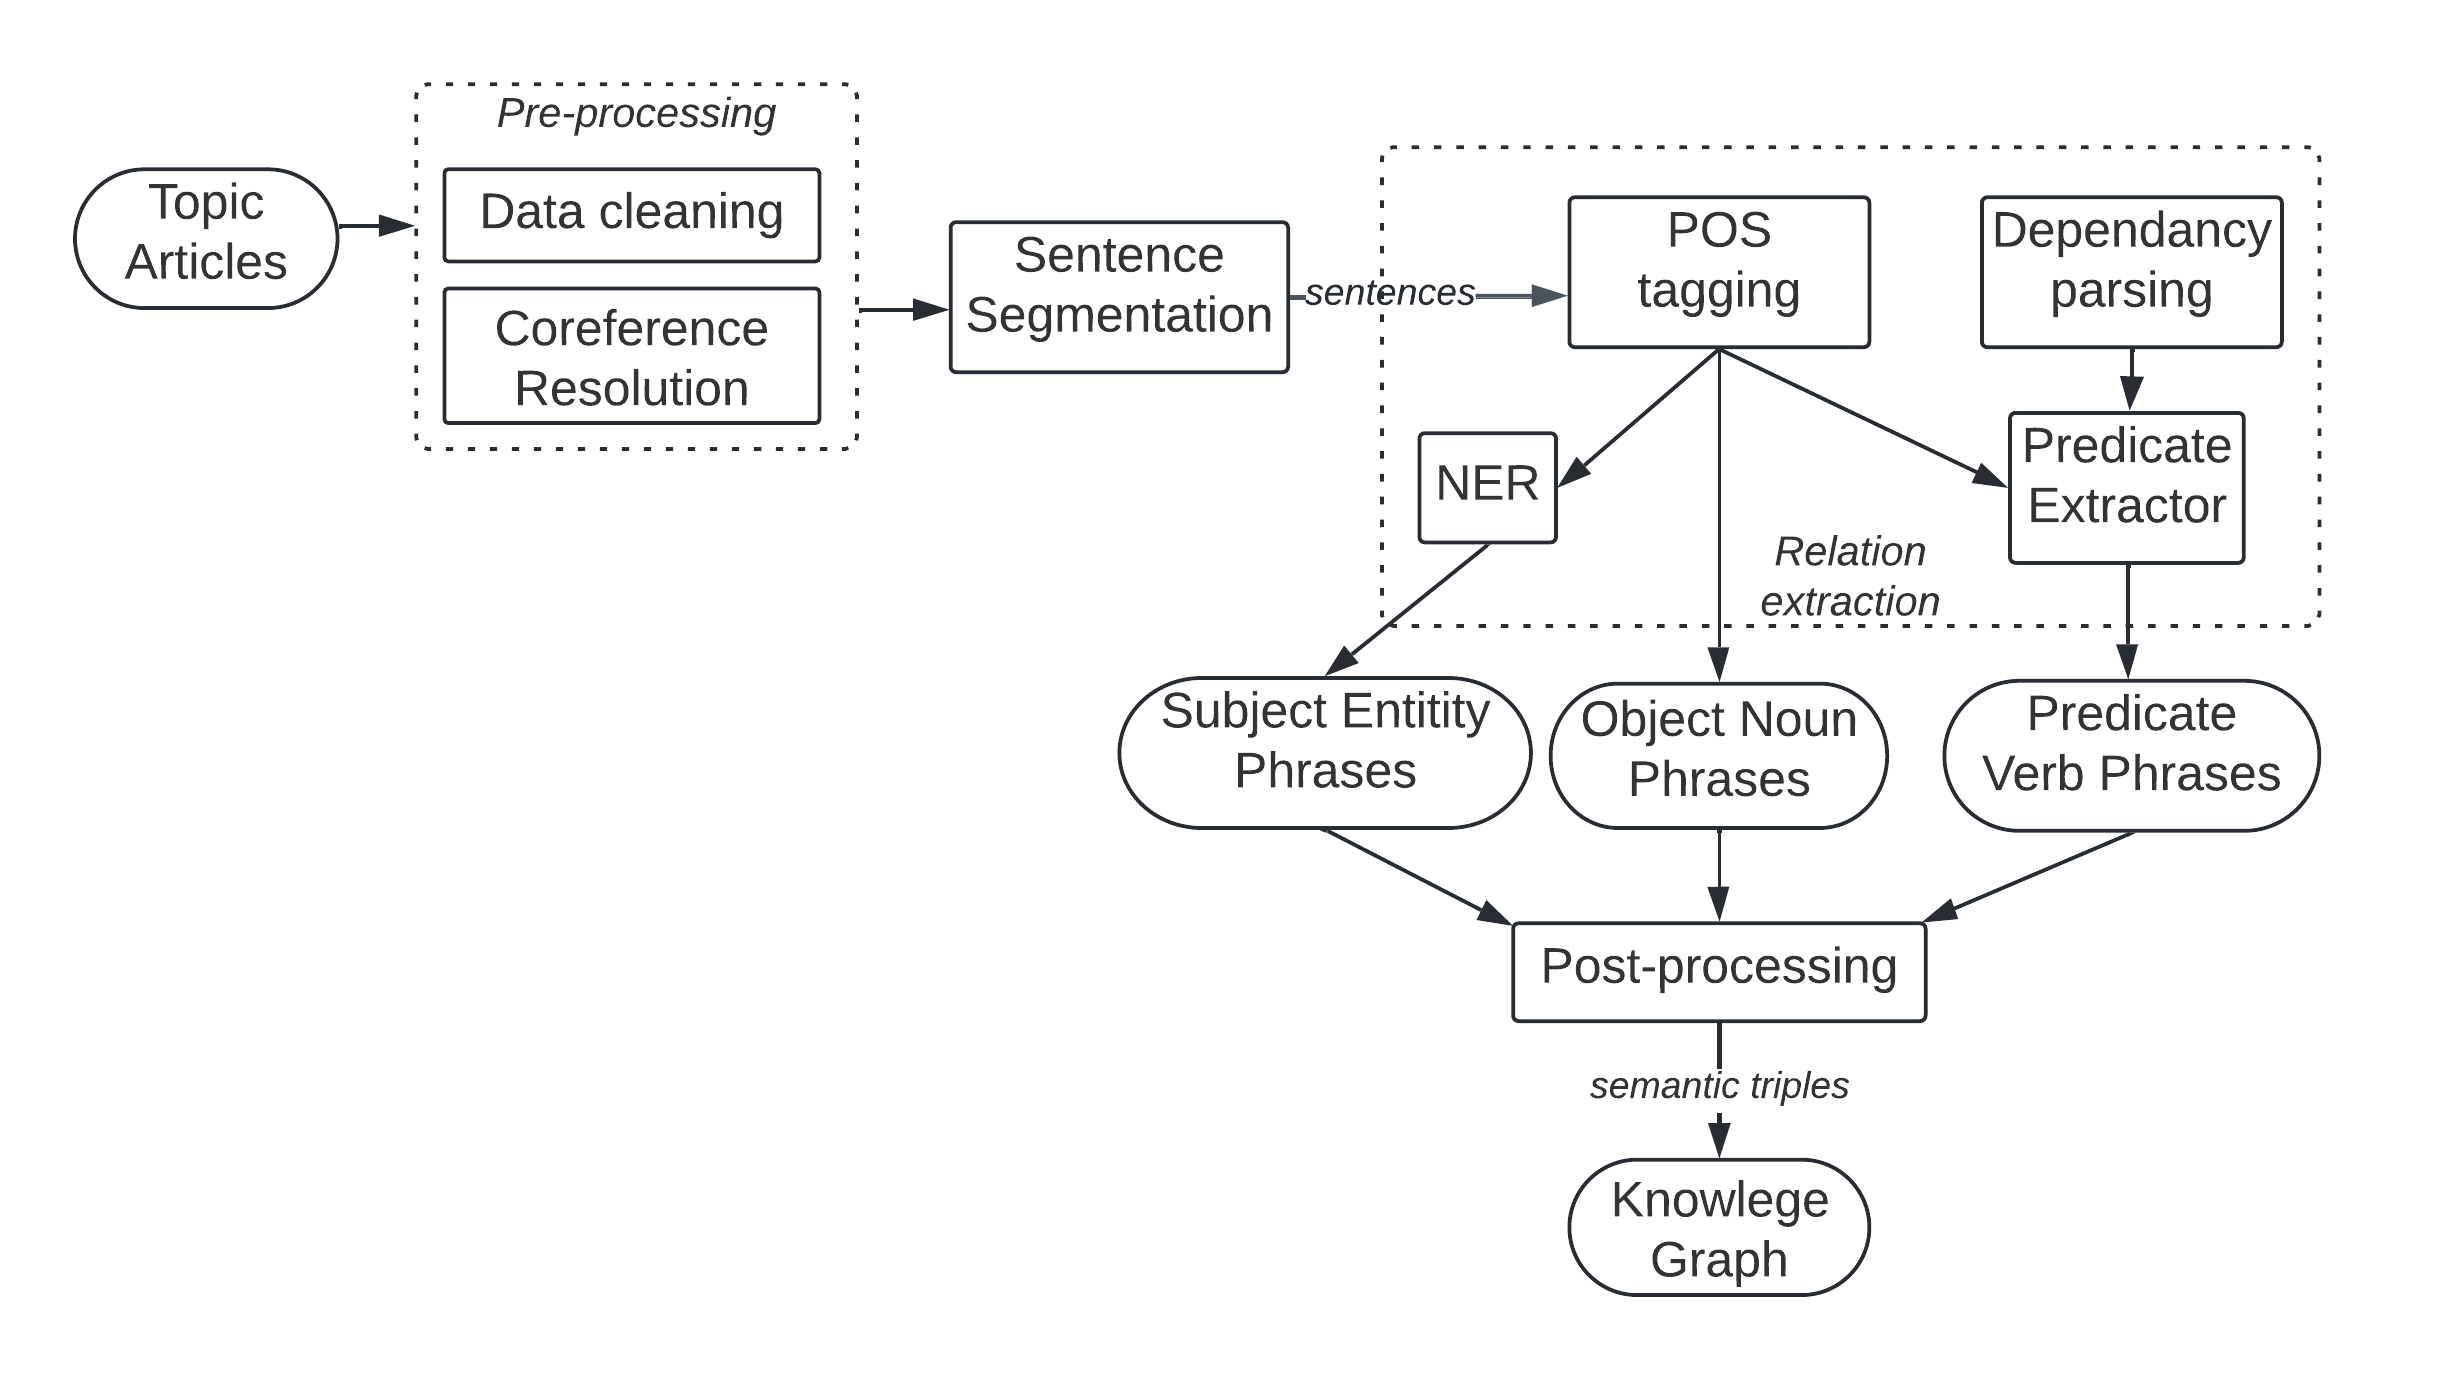
\includegraphics[scale=0.15]{images/ste_imp.png}
  \vspace{-2ex}
  \caption{Overview of Semantic Triple Extraction}
  \label{fig:rel_overview}
\end{figure}

\subsection*{Processing Articles}
As seen in~\Cref{fig:rel_overview}, before any information extraction, we need to ensure that the data is correctly preprocessed. For this, the coreference resolved, cleaned articles from  \Crefrange{coref}{data_cleaning} are used. This ensures that all pronouns corresponding to the named entities are resolved, allowing more triples to be extracted from the article corpus with named entities as the `subject'. Extracting triples on a `cleaned' article corpus gets rid of unnecessary text, including stopwords, \hl{allowing the model to focus on `semantically rich' words which provide more context in a smaller set of words}. Each topic article then undergoes sentence segmentation (via spaCy \texttt{SentenceSplitter}) to obtain a list of sentences from which triples can be extracted.

\subsection*{Extracting Predicate}

As discussed in \Cref{key_decisions_rel}, the predicate phrases would be extracted as verb phrases. This is done by regex matching of part-of-speech (POS) tags (refer to Appendix \Cref{appendix:pos}) as seen below. 

\begin{minted}[fontsize=\footnotesize, breaklines=True, frame=lines,
  framesep=1mm, baselinestretch=1.0]{python}
verb_patterns = [
  [{'POS':'AUX', 'OP':'?'}, {'POS':'PART', 'OP':'?'}, {'POS':'VERB', 'OP':'+'}, {'POS':'ADP', 'OP':'+'}],
  [{'POS':'VERB', 'OP':'?'}, {'POS':'ADV', 'OP':'*'}, {'POS':'VERB', 'OP':'+'}]
  ]
\end{minted}

% \todonum[inline]{Talk about why these particular regex}

The above regex patterns do not limit the verb phrase to the `VERB' POS tag, but instead account for other relevant information such as auxiliary verbs (`AUX'), adverbs (`ADV') and adposition (`ADP') to be pulled from the sentences as candidate verb phrases in order to retain semantic context. These are then filtered to obtain the phrases where the `root' of the sentence is present. This is done using dependency parsing through the spaCy library. Generally, in dependency-based grammars, all words or tokens, in a sentence,  barring one,  are dependent on other words.  This is the root  of the sentence. Most commonly, this word a verb. Therefore, since the scope of relations extracted focuses on the predicate being a verb, the root verb is derived from the dependency tree and all verb phrases containing the root verb are retained. Given the regex pattern matching criteria discussed above, each sentence might result in multiple root verb phrases, for example, one with just the root verb (e.g 'calling'), one with the auxiliary verb (e.g. 'are'), root verb (e.g. 'calling') and adposition (e.g. 'for') as shown in~\Cref{verb_phrases}. In order to extract the most informative coherent relations, the longest verb phrase is selected. 

\begin{figure}[H]
\centering
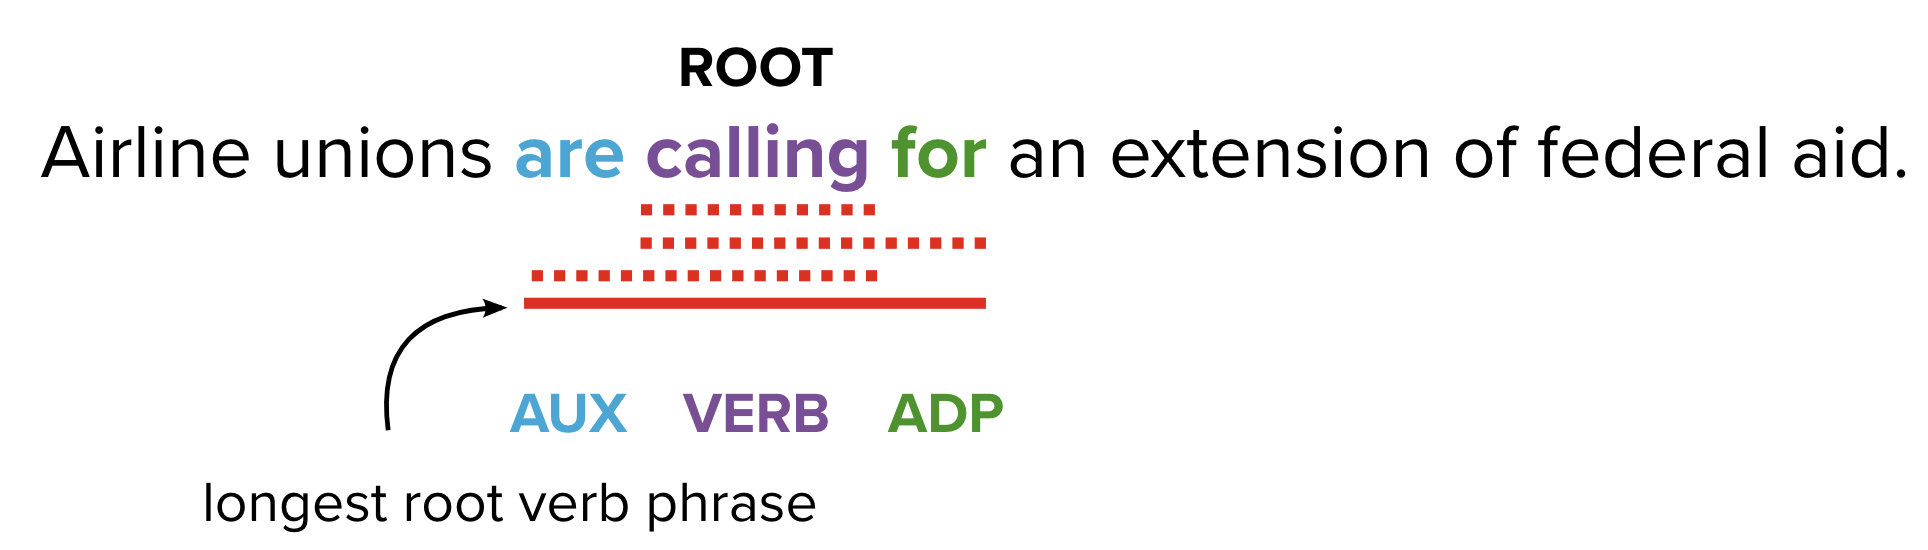
\includegraphics[scale=0.35]{images/verb_phrases.png}
\caption{Verb phrases extracted from an example sentence from article corpora}
\label{verb_phrases}
\end{figure}

\subsection{Extracting Subject and Object}
As discussed in \Cref{key_decisions_rel}, the `subject' and `object' are noun phrases (NP), particularly entity phrases for `subject'. Therefore, in order to derive these, the `noun chunks' are extracted from the sentence using POS tagging and chunking from the spaCy pipeline. These `noun chunks' are base noun phrases with no nested NP and relative clauses~\cite{spacy} and are returned as a list of \texttt{Spans}~\cite{spacy}, which are essentially slices of the sentence and contain information such as the `start' and `end' position of the sentence `chunk' (phrase). \Cref{alg:subject_relation} outlines the process of extracting the subject and object phrases in the semantic triple.

\begin{algorithm}[H]
  \caption{Outline of Triple Extraction Procedure}
  \label{alg:subject_relation}
  \begin{algorithmic}   
  \Function{GetSubjectAndAugmentedPredicate}{$verbPredicate, validEnts, nounPhrases$}
    \ForAll {$np \in nounPhrases$}
    
      \If {$np.start < verbPredicate.start$}
      \State $ents \gets n.containsAny(validEnts)$ 
      \Comment{all entities in np}
        \If {$ents.length == 0$}
        \State $continue$
        \EndIf
      \State $subjectEnt \gets ents.sort(key = lambda \ e: e.start)[0]$
      \State $remnantNp \gets np.partition(subjectEnt).last$ 
      \Comment remnant phrase right of subject
      \State $augmentedPred = remnantNp + verbPredicate $
      \State $break$
      \EndIf
    \EndFor
    \State \Return $subjectEnt, augmentedPred$
  \EndFunction

  \Function{GetObject}{$verbPredicate, nounPhrases$}
    \ForAll {$np \in nounPhrases$}
      \If {$np.start > verbPredicate.start$}
      \State $object \gets np$ 
      \State $break$
      \EndIf
    \EndFor
    \State \Return $object$
  \EndFunction
\end{algorithmic}
\end{algorithm}

\vspace{-3ex}
\subsubsection{Subject Entity and Augmented Predicate}
For the subject phrase, the noun phrases (NP) that occur before (to the left of) the verb phrase (`predicate') as well as contain any of the selected set of named entities, \texttt{valid\_entities}, are chosen as \texttt{subject candidates}. These \texttt{valid\_entities} are derived by performing Named Entity Recognition (NER) on the sentence using the Fine-Grained NER model as detailed in~\Cref{alg:named_ents}. As mentioned previously in~\Cref{s:models}, the model returns 16 semantic types (refer to \Cref{appendix:semantic_types}). Some of these entity types can result in unnecessary and irrelevant triples with, for instance, (`two', \texttt{`CARDINAL'}) as the subject node. Therefore, in a slight adjustment to~\Cref{alg:named_ents}, a set of \texttt{ignore\_entity\_types}, containing \texttt{`DATE', `TIME', `CARDINAL', `PERCENT'} and \texttt{`QUANTITY'}, is passed to omit extracted entities of these types. This does not mean that information about these entities is completely ignored as they are likely to be extracted as object phrases when in reference to a `valid' subject named entity. 

Of the \texttt{subject candidates}, the first occurring (based on position of \texttt{Span}) is selected as the subject phrase. As mentioned \Cref{key_decisions_rel}, the aim is to have just the named entity as the `subject' to facilitate connectivity of triples in the KG. However, we do not lose the other semantic information in the subject phrase. Therefore, the subject phrase is split into the entity and the remnant phrase \textit{after} the entity, which is then prepended to the predicate. This way the information conveyed by the noun phrase is conserved, but the subject nodes are maintained as an entity. For example, for the triples: \texttt{(`Transat investors', `choose receiving', `cash payment')} and \texttt{(`Transat', `to become part of', `Air Canada')}, splitting the $1^{st}$ triple's subject to get `Transat' and `investors' and augmenting the predicate with the latter to get the updated triple: (`Transat', `investors choose receiving', `cash payment'). \Cref{fig:transat_before} and \Cref{fig:transat_after} show the KG snippet for these triples before and after splitting the subject phrase respectively.
  
\begin{figure}[H]
  \begin{minipage}{0.4\linewidth}
  \centering
  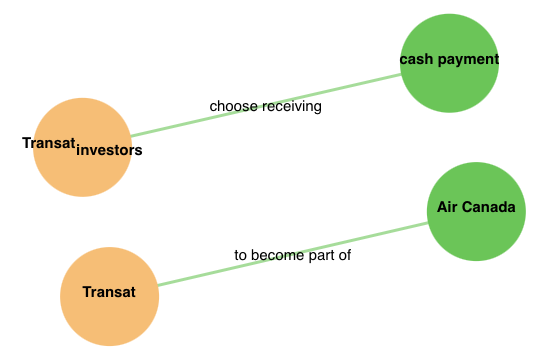
\includegraphics[width=\linewidth]{images/kg_transat.png}
  \caption{KG snippet before predicate augmentation}
  \label{fig:transat_before}
  \end{minipage}
  \hfill
  \begin{minipage}{0.4\linewidth}
  \centering
  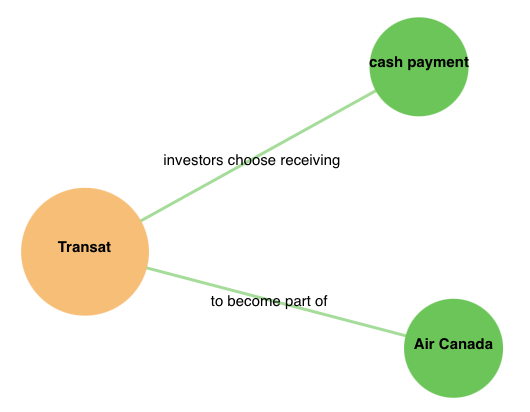
\includegraphics[width=\linewidth]{images/kg_transat_correct.png}
  \caption{KG snippet after predicate augmentation}
  \label{fig:transat_after}
  \end{minipage}
\end{figure}

\subsubsection{Get object phrase}
Getting the object is fairly simple as shown in \Cref{alg:subject_relation} and involves getting the first (closest in position) `noun phrase' after the `predicate' (the longest root verb phrase).

\subsubsection{Post-processing}
Once the semantic triples are obtained from the article corpus for each topic, the triples are filtered. After ensuring the that all components of the triple are not null, the triples where the relations/predicates contains words like "said" and "told" in their different forms are filtered. This is done because, often in news articles, direct quotes are made by entities and the relation extraction engine retrieves some poor relations that do not add to the quality of the relations extracted for a particular entity. Furthermore, in order to ensure conciseness of the triples and eliminate redundancy, any common substring (likely to occur from noun phrase chunking and verb phrase regex matching) is eliminated by calculating the \hl{longest common substring containing complete words} between the subject and object as well as (augmented) predicate and object and removing it from the object phrase. 


\section{Results and Discussion}

Once the qualifying semantic triples for each topic are obtained, these are passed to the visualisation engine. An example of the semantic relations extracted for the topics for a given cluster in Business 2021 is shown in \hl{Figure ??}

% \todonum[inline]{Show types of relations extracted with dep parsing and otherwise}
% \todonum[inline]{Talk about the object-relation-subject gotcha.}

This particular method avoids the stringent dependency of the "subject" and "object" phrases on their actual dependency positions in the grammar, This is because given the nature of news articles, the sentence structure is relatively complex with several different subjects and objects. For the knowledge graph, ultimately, the relations extracted need to focus around different named entities. Relying on the dependency grammar structure to find the subject and object dos not hold as in a given sentence, the structure of the sentence heavily influences the information extracted. This means that more often than not, relevant information about entities is lost due to the entity not necessarily having one of \texttt{"nsubj", "csubj", "nsubjpass",	"csubjpass"} as the dependency. 

\subsection*{Limitations}
verb-based approaches can only extract a
single relation embedded in a sentence composed of a verb
phrase sandwiched between two entities of interest. 
However, current verb-based approaches can only extract a
single relation embedded in a sentence composed of a verb
phrase sandwiched between two entities of interest. 



